% arara: pdflatex: { shell: yes }
% arara: bibtex
% arara: pdflatex: { shell: yes }
% arara: clean: { files: [Expo.Tesis.aux, Expo.Tesis.log, Expo.Tesis.nav, Expo.Tesis.out, Expo.Tesis.snm, Expo.Tesis.toc, Expo.Tesis.idx, Expo.Tesis.ilg, Expo.Tesis.ind, Expo.Tesis.vrb, Expo.Tesis.fdb_latexmk, Expo.Tesis.pyg]}
\documentclass[compress]{beamer}
\mode<presentation>

\usetheme{Warsaw} % Beamer Theme
\useoutertheme{infolines}
\useinnertheme{circles} % Beamer inner Theme
\setbeamertemplate{navigation symbols}{}
\renewcommand{\figurename}{Figura}
\setbeamertemplate{frametitle continuation}{}%\insertcontinuationcount
%\usepackage{beamerinnerthemecircles}
% inner themes include circles, default, inmargin, rectangles, rounded
%\usepackage{beamerouterthemesmoothbars}
%\useoutertheme[subsection=false]{smoothbars}

%%%%%%%%%%%%%%%%%%%%%%%%%%%%%%%%%%%%%%%%%%%%%%%%%%%%%%%%%%%%%%%%%%%%%%%%%%%%%%%%%%%%%%%%%%
%%%%%%%%%%%%%%%%%%%%%%%%%%%%%%%% Use packages %%%%%%%%%%%%%%%%%%%%%%%%%%%%%%%%%%%%%%%%%%%%
%%%%%%%%%%%%%%%%%%%%%%%%%%%%%%%%%%%%%%%%%%%%%%%%%%%%%%%%%%%%%%%%%%%%%%%%%%%%%%%%%%%%%%%%%%
\usepackage{subfigure}
\usepackage{multicol}
\usepackage{amsmath}
\usepackage{epsfig}
\usepackage{graphicx}
\usepackage[all,knot]{xy}
\xyoption{arc}
\usepackage{url}
\usepackage{multimedia}
\usepackage{hyperref}
\usepackage[utf8x]{inputenc}
\usepackage{enumerate}
\usepackage{comment}
%%Pygments%%
\usepackage{fancyvrb}
\usepackage{xcolor}
\definecolor{SkyblueDark}{HTML}{204A87}
\setbeamercolor{frametitle}{fg=white}
\setbeamercolor{structure}{fg=SkyblueDark}
%%%%%%%%%%%%%%%%%%%%%%%%%%%%%%%%%%%%%%%%%%%%%%%%%%%%%%%%%%%%%%%%%%%%%%%%%%%%%%%%%%%%%%%%%%
%%%%%%%%%%%%%%%%%%%%%%%%%%%%%% Title Page Info %%%%%%%%%%%%%%%%%%%%%%%%%%%%%%%%%%%%%%%%%%%
%%%%%%%%%%%%%%%%%%%%%%%%%%%%%%%%%%%%%%%%%%%%%%%%%%%%%%%%%%%%%%%%%%%%%%%%%%%%%%%%%%%%%%%%%%

\title{Plataforma web para el an\'alisis de la gesticulaci\'on facial}
%\subtitle{POO}
\author[Jaime Jes\'us Delgado Meraz]{Jaime Jes\'us Delgado Meraz\\{\small Advisor: Pedro Luis S\'anchez Orellana}}
\date{Agosto 2013}
\institute[ITCV]{Maestr\'ia Profesionalizante en Sistemas Computacionales\\Divisi\'on de Estudios de Posgrado de Investigaci\'on\\Instituto Tecnol\'ogico de Ciudad Victoria}

%%%%%%%%%%%%%%%%%%%%%%%%%%%%%%%%%%%%%%%%%%%%%%%%%%%%%%%%%%%%%%%%%%%%%%%%%%%%%%%%%%%%%%%%%%
%%%%%%%%%%%%%%%%%%%%%%%%%%%%%% Begin Your Document %%%%%%%%%%%%%%%%%%%%%%%%%%%%%%%%%%%%%%%
%%%%%%%%%%%%%%%%%%%%%%%%%%%%%%%%%%%%%%%%%%%%%%%%%%%%%%%%%%%%%%%%%%%%%%%%%%%%%%%%%%%%%%%%%%
\begin{document}
%%%%%%%%%%%%%%%%%%%%%%%%%%%%%%%%%%%%%%%%%%%%%%%%%%%%%%%%%%%%%%%%%%%%%%%%%%%%%%%%%%%%%%%%%%
\frame{\titlepage}
%%%%%%%%%%%%%%%%%%%%%%%%%%%%%%%%%%%%%%%%%%%%%%%%%%%%%%%%%%%%%%%%%%%%%%%%%%%%%%%%%%%%%%%%%%
%\section[Outline]{}
%\frame{\tableofcontents}
\AtBeginSection[]
{
  \begin{frame}
    %\frametitle{Table of Contents}
%    \begin{multicols}{2}
	\tableofcontents[currentsection]
%	\end{multicols}
  \end{frame}
}
%%%%%%%%%%%%%%%%%%%%%%%%%%%%%%%%%%%%%%%%%%%%%%%%%%%%%%%%%%%%%%%%%%%%%%%%%%%%%%%%%%%%%%%%%%
\section{Introduction}
\begin{frame}
	\frametitle{What is Face Analysis?}
	\begin{itemize}
	\item The analysis of facial expressions constitutes a critical and complex portion of our non-verbal social interactions.
%	\item It is important to consider that facial expression recognition is different from facial expression analysis
	\end{itemize}
	\begin{description}
	\item[Facial Expression Recognition] is focused on classification of the structure of the face into a set of general emotions.
	 \item[Facial Expresion Analysis] is focused on meassuring how these emotions are produced in the face.
	\end{description}
\end{frame}

\begin{frame}
		\begin{figure}
		\centering
		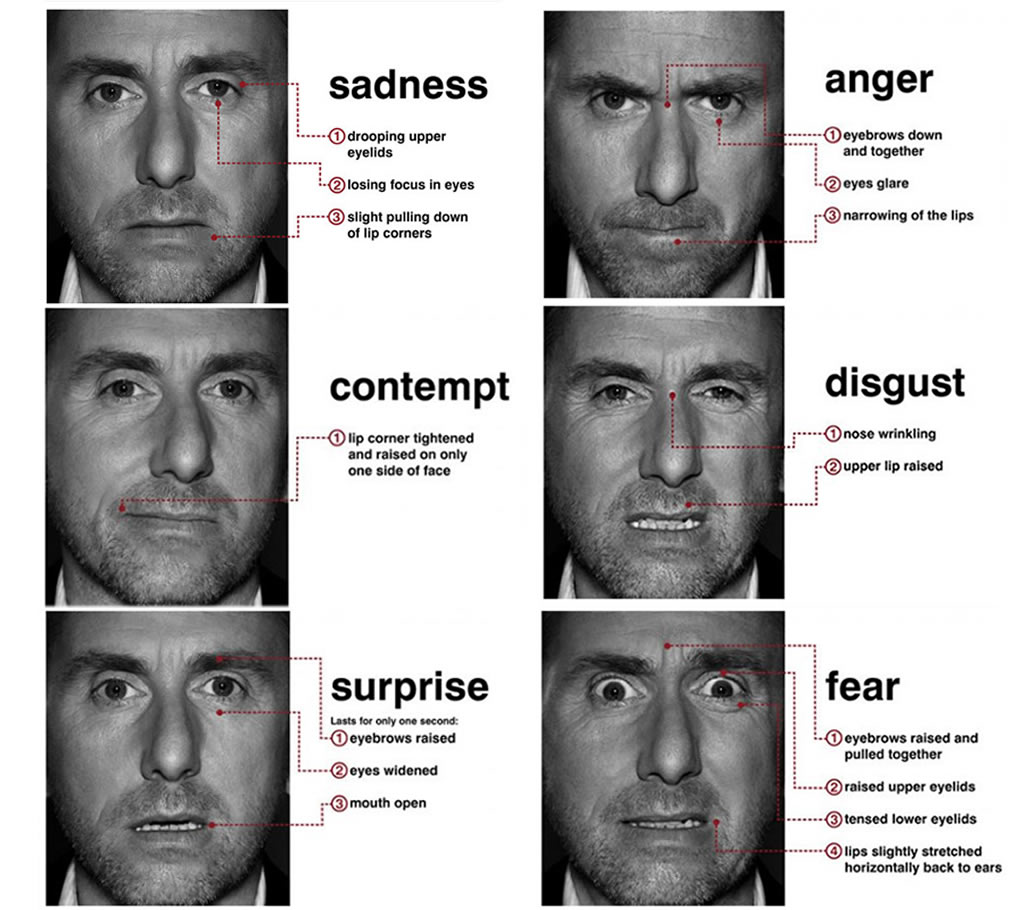
\includegraphics[scale=0.3]{img/microexpressions2.jpg}
	\end{figure}
\end{frame}

\begin{frame}
	\frametitle{Facial Gestures Recognition}
	\begin{itemize}
	\item There are three main steps for working in facial gestures recognition:
		\begin{enumerate}
		\item Face detection,
		\item Extraction of facial gestures information, and
		\item Classification of the information extracted.
		\end{enumerate}.
	\item The methods for facial gesture analysis can be grouped in \textbf{deformation} extraction and \textbf{motion} extraction.
	\end{itemize}
\end{frame}

\subsection{Motivation}
\begin{frame}
	\frametitle{Motivation}
	\begin{itemize}
	\item Human interaction is very important in many different aspects in our daily life, such as business meeting, medical diagnostics, etc.
	\item However, thanks to the improvement of technology, this operations can be done remotely, which can be especially useful when the distance is considered a barrier, but this producess another problem which is the lack of physical gesture apreciation.
%	\item To solve this issue, we propose the use of a web service that allows to remotely evaluate gestures.
	\end{itemize}
\end{frame}

\begin{frame}
	\begin{figure}
		\centering
		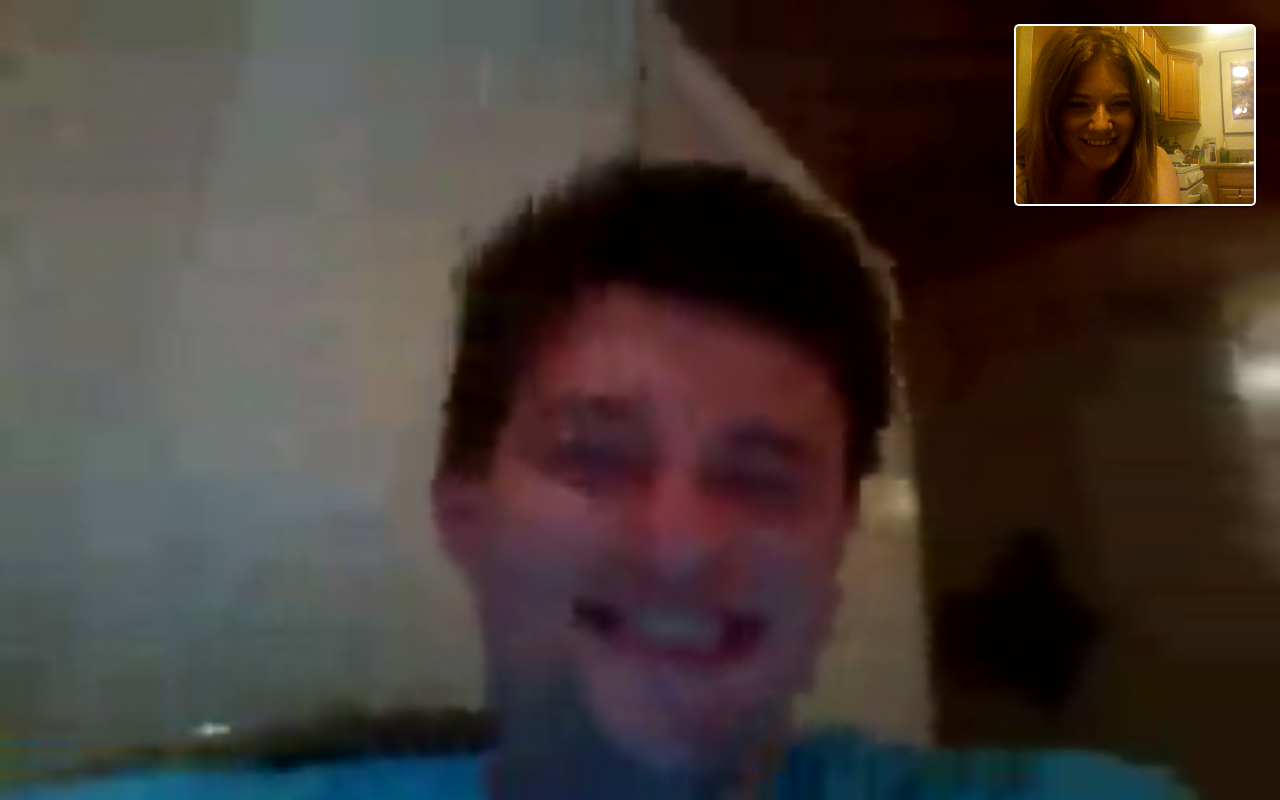
\includegraphics[scale=0.2]{img/pixelated.png}
		\caption{Example of the lack of physical gesture apreciation}
	\end{figure}
\end{frame}

\subsection{Problem Statement}
\begin{frame}
	\frametitle{Problem Statement}
	\begin{alertblock}{Problem}
	Given a sequence of images from the face, taken in a client computer, where the illumination conditions and background motion are restricted, the problem of analyzing facial gestures on the web, could be stated as an architecture that allows transmission of compressed images through a web service, in order to produce an analysis of facial gestures.
	\end{alertblock}

	\begin{itemize}
		\item From this we state the following research questions:
		\begin{enumerate}
			\item Considering the speed of internet connections in M\'exico, what techniques can be used to increase the speed of image transfer?
			\item Which type of web service is more suitable for image transmission/analysis?
		\end{enumerate}
	\end{itemize}
\end{frame}

\subsection{Objectives}
\begin{frame}
	\frametitle{Objectives}
	\begin{block}{General}
	Design a web architecture that allows the efficient transmission of facial image sequences to compute an analysis about the behaviour of facial gesticulations, in order to obtain symmetrical / asymmetrical motion patterns which might be used for the decision-making process.
	\end{block}
\end{frame}

\begin{frame}
	\frametitle{Objectives}
	\begin{block}{Specific}
		\begin{enumerate}
		\item Implement an image compression technique that allows fast Internet broadcasting.
		\item Design and implement a web architecture for the reception and decompression of compressed images.
		\item Adapt a given algorithm for the analysis of gesticulations in the transmitted images.
		\item Design a set of experiments to test the web architecture.
		\end{enumerate}
	\end{block}
\end{frame}

\subsection{Scope and Constraints}
\begin{frame}
	\frametitle{Scope and Constraints}
	\begin{itemize}
	\item The proposed architecture focuses only on the compression-transmission process of images, and does not consider the motion from other regions of the body.
	\item Moreover, the mechanisms for the analysis of the image sequences were generated in collaboration with researchers of the Universidad Polit\'ecnica de Victoria and were only used, but not implemented.
	\end{itemize}
\end{frame}

\section{State of Art}
\begin{frame}
	\frametitle{Facial Gesture Analysis Techniques}
	\begin{itemize}
	\item The analysis problem has been approached from two main streams~\cite{Fasel2003}: facial deformation extraction models and facial motion extraction models (both 2D or 3D).
%	Motion extraction approaches directly focus on facial changes produced by facial expressions, whereas deformation-based methods contrast the visual information against face models to extract features product of expressions and not by age deformation like wrinkles.
	\item \textbf{2D based techniques}.\\Advantages: fast processing. Disadvantages: very large training data sets is needed to model environment variations.
	\item \textbf{3D based approaches}.\\Advantages: higher accuracy \cite{Fang2012}. Disadvantages: Higher computational complexity.
	\end{itemize}
\end{frame}

\begin{frame}
	\begin{itemize}
	\item Therefore...
	\end{itemize}
	\begin{figure}[h]
    \centering
    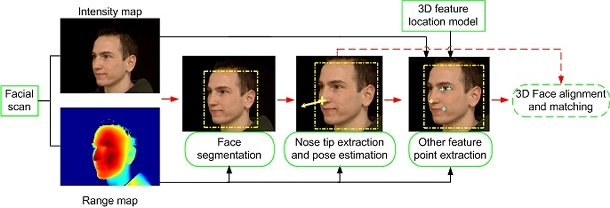
\includegraphics[scale=0.7]{img/featuresExtraction.jpg}
%    \caption[Basic human emotions and Facial gesture analysis]{(A) Basic human emotions. (B) Facial gesture analysis.}
	\end{figure}
\end{frame}

\subsection{Neural Networks}
\begin{frame}
	\frametitle{Spiking Neural Networks}
	\begin{figure}[h]
    \centering
    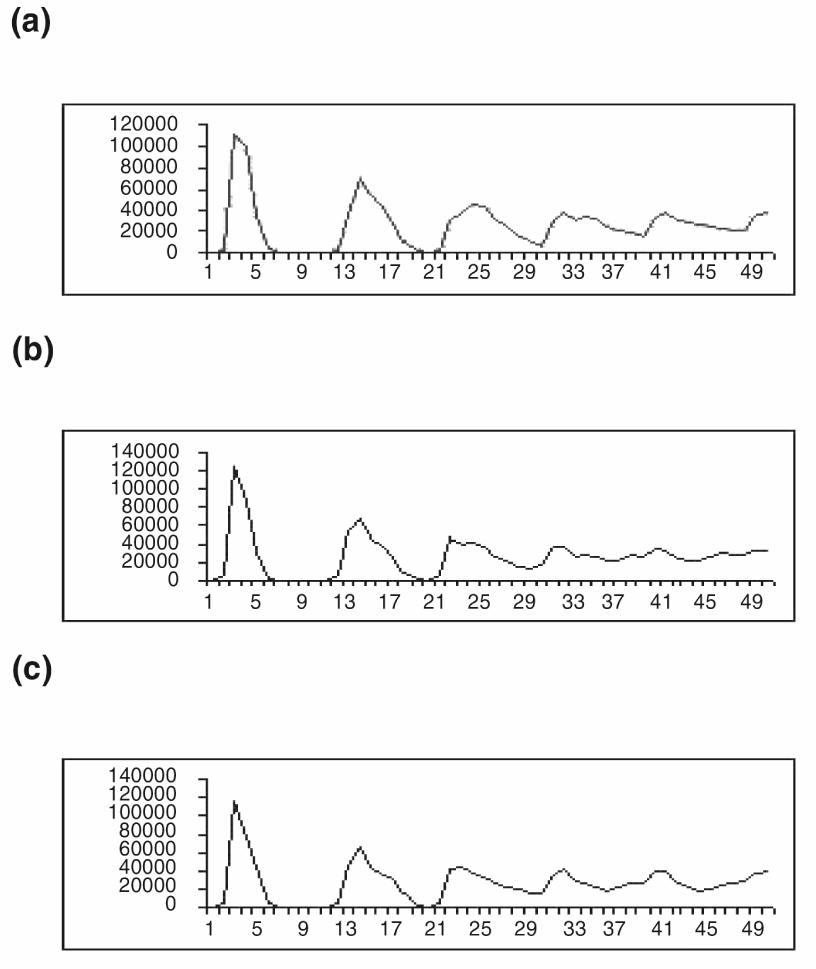
\includegraphics[scale=0.7]{img/snn.png}
    \caption{Obtained results: (a) Left-Right Eyes, (b) Left-Right Nose, (c)Left-Right Mouth}
	\end{figure}
\end{frame}
\subsection{Web Services}
\begin{frame}
	\frametitle{Web Services}
	\begin{itemize}
	\item SOAP: Simple Object Access Protocol \cite{Pautasso:2007}. It was designed to be a platform and language-neutral alternative to previous middleware technologies.
	\item REST: Representative State Transfer \cite{Fielding00Phd}. A later evolution to SOAP disadvantages.
	\end{itemize}
\end{frame}

\subsection{Image Compression}
\begin{frame}
	\frametitle{}
	\begin{itemize}
	\item Since 3D images are heavier, it is necessary to implement an image compression technique. Basically they can be divided into:
	\item Lossless Compression Tecniques: The feature of the lossless compression technique is that the original image can be perfectly recovered from the compressed image \cite{Woods:2008} (such as Run length encoding, Huffman encoding, etc.).
	\item Lossy Compression Technique provide higher compression ratio than lossless compression (such as Vector quantization, Fractal coding, etc.).
	\end{itemize}
\end{frame}

\subsection{Experimental Designs}
\begin{frame}
	\begin{itemize}
	\item The experimental design is a key piece in the software development process given that it allows identifying failures in the software before it begins to operate.
	\item An alternative strategy to test software is the use of Covering Arrays (CAs).
	\item A Covering Array is a combinatorial object that, with a small number of cases, covers a certain level of interaction of a set of parameters \cite{Kuhn:2008}.
	\end{itemize}
\end{frame}

\begin{frame}
	\begin{itemize}
	\item A covering array is an $N \times k$ matrix over an alphabet $v$ each $N \times k$ subset contains at least one time each combination from ${0,1,\ldots,v−1}^{t}$, given a positive integer value $t$.
	\end{itemize}
\end{frame}

\begin{frame}
	\begin{itemize}
	\item Covering Arrays have been an object of study and application in different research areas. Cawse \cite{Cawse:2003} used CAs in the material design, Hedayat et al. \cite{Hedayat:1999} used them in medicine and agriculture.
	\end{itemize}
\end{frame}

\section{Methodology}
\begin{frame}
	\frametitle{Methodology}
	\begin{description}
\item[1st Stage] In this stage, the different techniques for image compression/decompression were studied, in order to choose a set of them to be implemented and tested. Once the implementations of the selected techniques were made, they were tested and compared to choose one that was integrated into a client application. This client application is responsible of capturing the images for their compression by the selected technique.
\end{description}
\end{frame}

\begin{frame}
	\frametitle{Methodology}
	\begin{description}
\item[2nd Stage] In this stage, the different approaches for web services were analyzed, to choose the most appropriate solution for the problem to be solved. Also, a local web server was mounted, in order to implement the chosen web service model. Once the web service was implemented, the decompression technique to reverse the technique selected on the previous stage, was setup on the web service, this, in order to connect the client to the server to send the compressed images, and then testing the process of transmission-reception-decompression. Based on the results from the previous tests, the necessary adjustments were made to ensure both the proper functioning of the connection between the client and server, and the reception of the original image as captured by the client.
\end{description}
\end{frame}

\begin{frame}
	\frametitle{Methodology}
	\begin{description}
\item[3rd Stage] In this stage, the work was focused on the adaptation of the algorithm for facial gestures analysis, since it was originally developed to work in a local environment. This adaptation included a mechanism to interact with the compression/decompression technique previously developed, and a mechanism to retrieve and process the results from the facial gesture analysis algorithm, also, a user interface for displaying the results of the analysis was created.
\end{description}
\end{frame}

\begin{frame}
	\frametitle{Methodology}
	\begin{description}
\item[4th Stage] In this stage, the work was focused on the adaptation of the algorithm for facial gestures analysis, since it was originally developed to work in a local environment. This adaptation included a mechanism to interact with the compression/decompression technique previously developed, and a mechanism to retrieve and process the results from the facial gesture analysis algorithm, also, a user interface for displaying the results of the analysis was created.
\end{description}
\end{frame}

\begin{frame}[t,allowframebreaks]\frametitle{Results}

\end{frame}

\begin{frame}[t]\frametitle{Conclusion}
\end{frame}

\begin{comment}
\section{Schedule}
\begin{frame}
	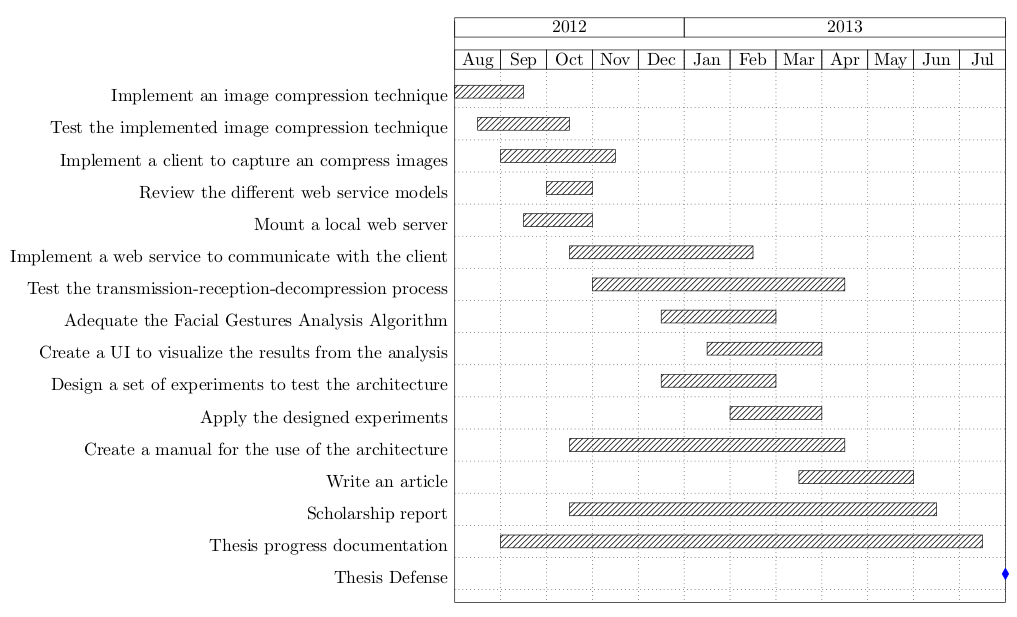
\includegraphics[scale=0.30]{img/schedule.png}
\end{frame}

\section{Infraestructure}
\begin{frame}
	\frametitle{Infraestructure}
	\begin{itemize}
	\item Laptop HP Pavilion DV5-1135la
		\begin{description}
		\item[OS] Ubuntu Linux 11.10 (32 bits).
		\item[Microprocessor] AMD Turion X2 Dual-Core Mobile Processor RM-72 (2.1 GHz).
		\item[Memory] 3072MB 800MHz DDR2 System Memory (2 Dimm).
		\item[Video Graphics] ATI Radeon HD 3450 Graphics (1533MB total graphics memory with 256MB dedicated).
		\item[Hard Drive] 320 GB (5400 RPM).
		\item[Webcam] Webcam HP Pavilion (VGA low-light)
			\begin{description}
			\item[Resolution] $648 \times 480$.
			\item[FPS] 30 fps.
			\end{description}
		\end{description}
	\item Both the client and the server, will be developed on open source software.
	\end{itemize}
\end{frame}
\end{comment}

\section{References}
\begin{frame}[allowframebreaks]{References}
\beamertemplatebookbibitems
\bibliographystyle{acm}
%\bibliographystyle{plainnat}
\bibliography{Tesis}
\end{frame}

\end{document}
